% BEGIN SECTION 3 - MIE
% Last updated by Milan Ilnyckyj 2013-06-24



		\singlespacing
		\section{The activities of fossil fuel companies are socially injurious, and this social injury cannot be reasonably remedied through shareholder voice}
		\label{sec:SocialInjury}
		\doublespacing



	\subsection{From the U of T divestment policy}



\begin{itquote}
Social injury is the injurious impact which the activities of a company are found to have on consumers, employees, or other persons, particularly including activities which violate, or frustrate the enforcement of, rules of domestic or international law intended to protect individuals against deprivation or health, safety, or basic freedoms
\end{itquote}



	\subsection{Social injury}


The primary activities of fossil fuel companies impose social injury on consumers, employees, or other persons.
The burning of a large portion of the world's reserves of fossil fuels would inflict great social injury through:
\begin{enumerate}
\item Impacts on agriculture
\item The inundation of coastal areas
\item Storms, droughts, other extreme weather
\item Wildfires
\item Increased risks to human health
\item Ecosystem collapse 
\item Threats to First Nations groups and indigenous cultures
\item Threats to the infrastructure of cities, including Toronto
\item The threat of abrupt and non-linear adverse climate impacts, arising from positive feedback effects and important thresholds in the climate system
\item Security implications
\end{enumerate}
In their 2007 report, the IPCC included a table that summarized how various forms of injury associated with climate change can be expected to worsen as the amount of warming increases:

% \begin{figure}
% 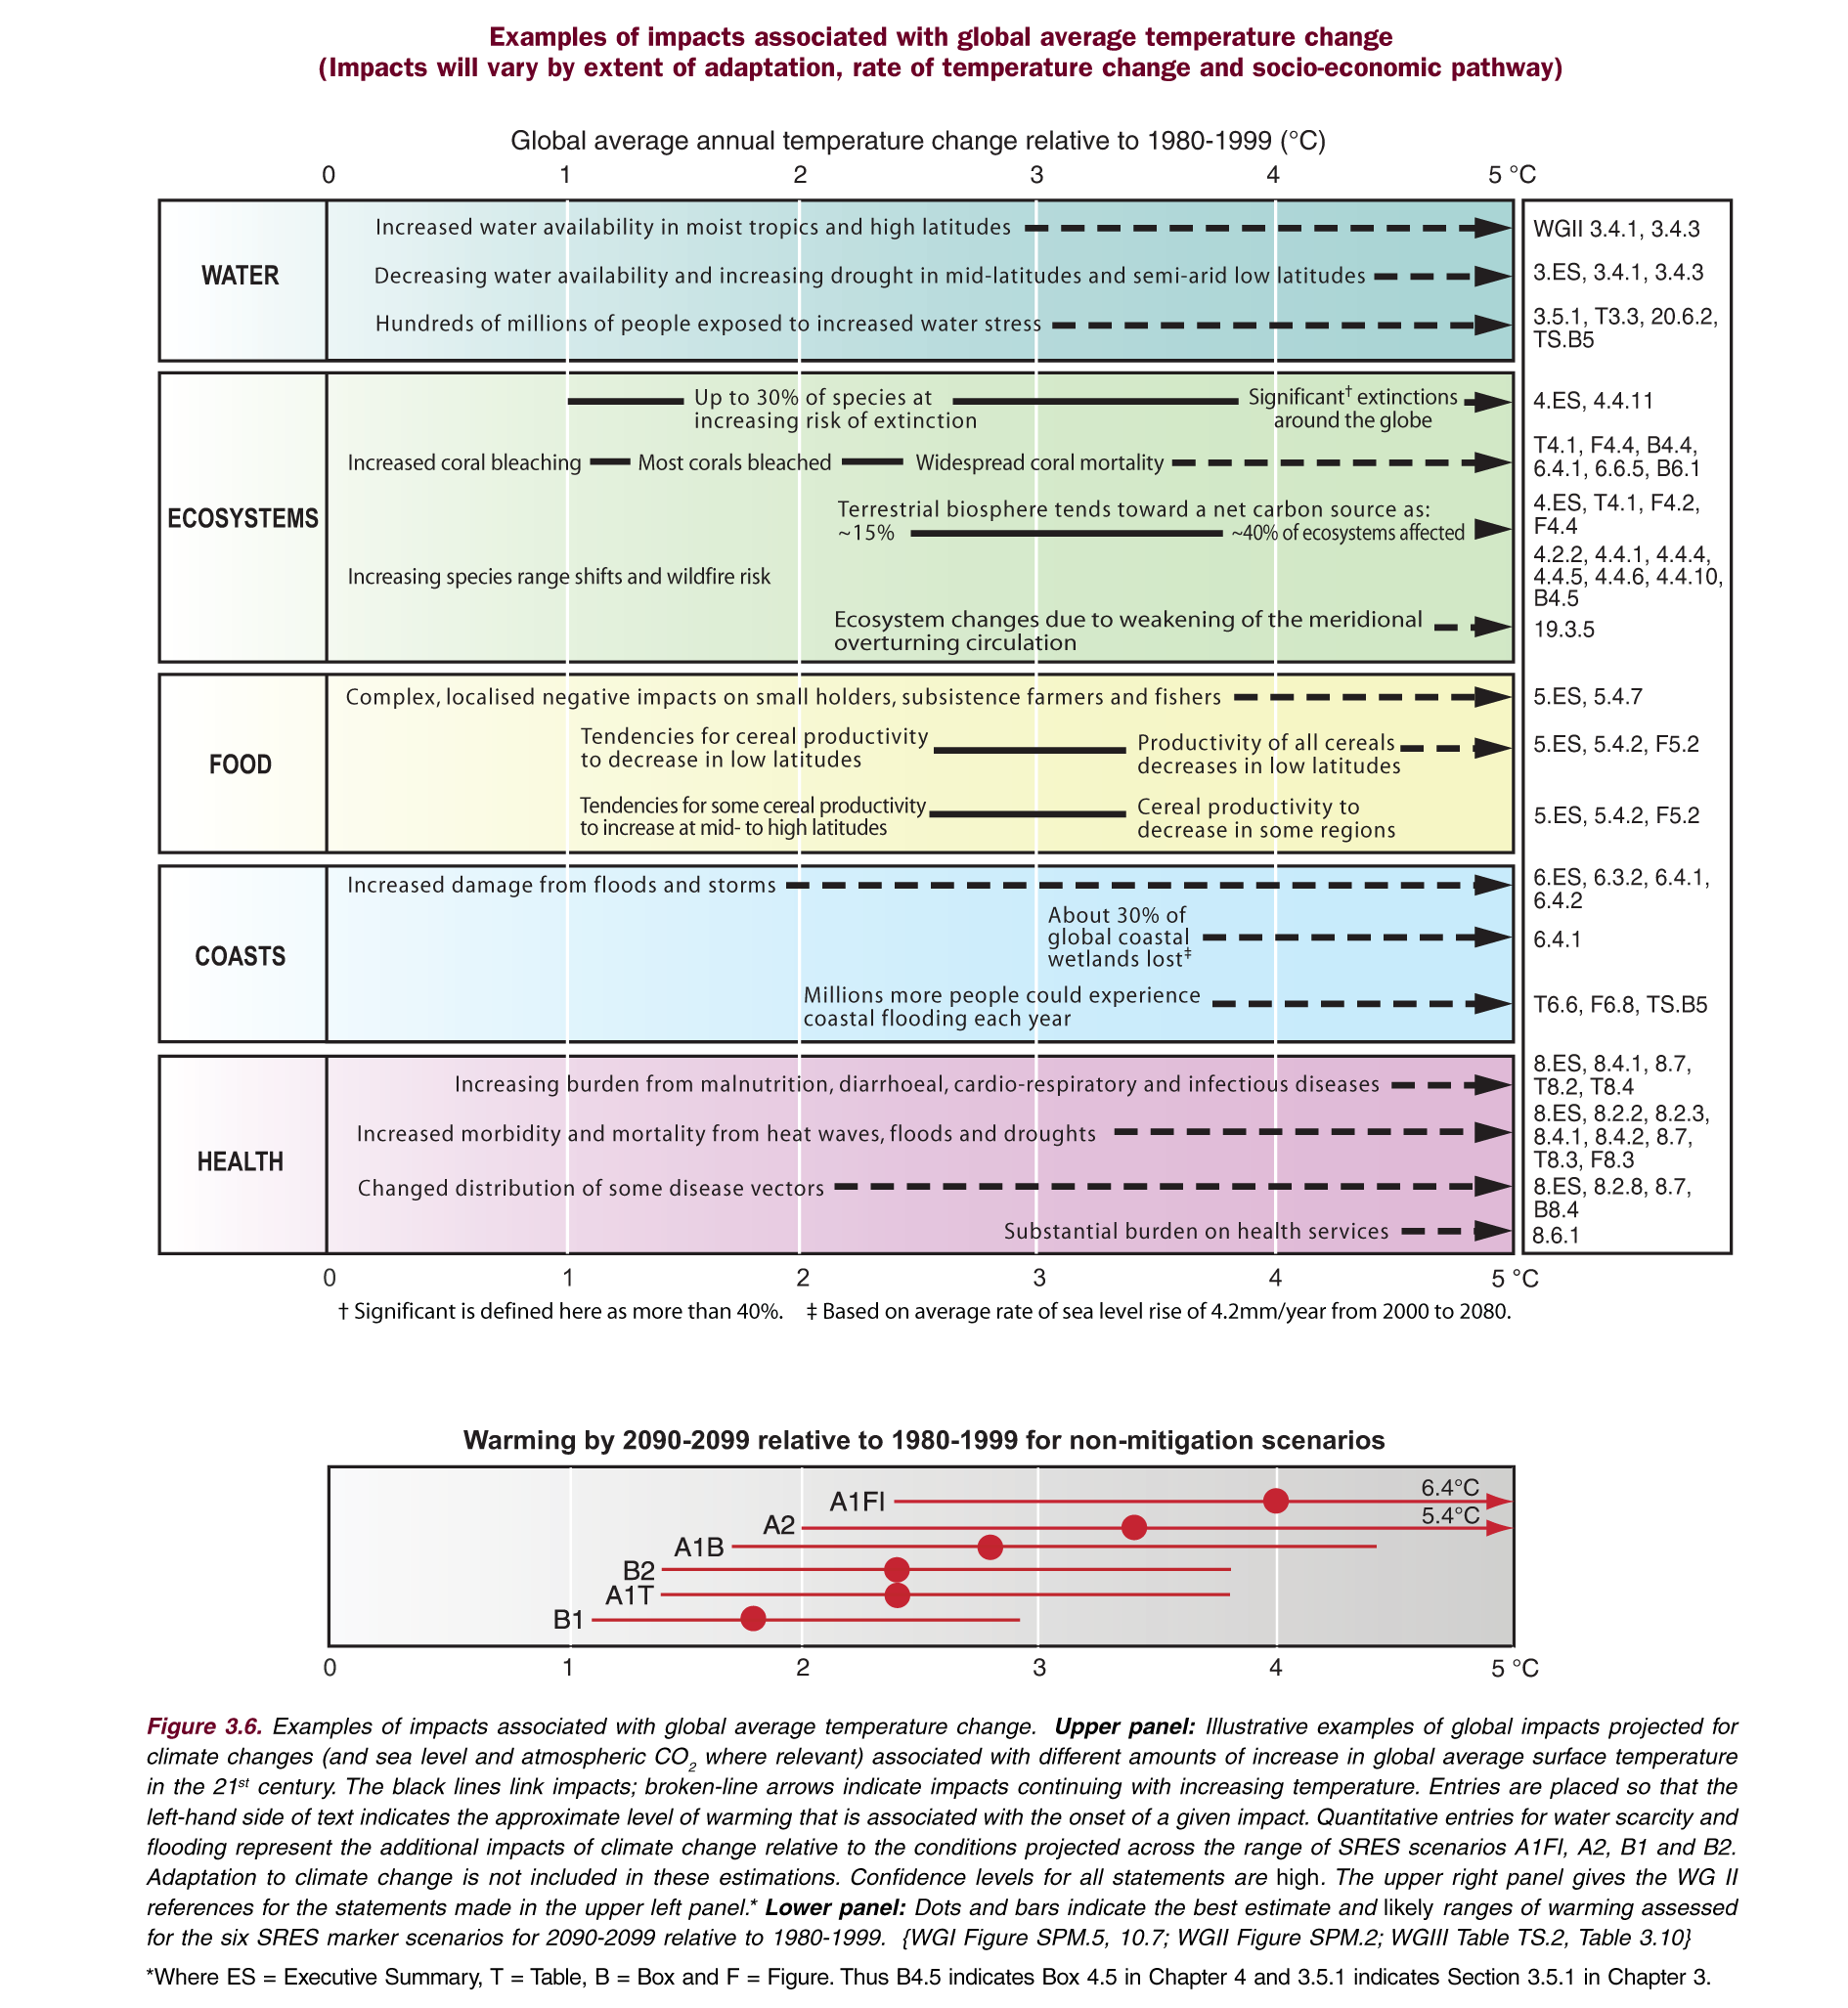
\includegraphics{s3-variousimpacts.png}
% \centering
% \caption{Examples of impacts associated with global average temperature change\footcite[][p.51]{IPCCar4_syr}}
% \end{figure}

Each of these impacts has consequences for human beings, and each represents a form of social injury being imposed on innocent people by the producers of fossil fuels.
According to the United Nations Development Programme, ``climate change... already imposes substantial costs, with the brunt of them borne by poor countries and poor communities''.\footcite[][p. 34]{UNHumanDev2013} \footcite[See also: ][]{WorldBankDevCC}
This harm is not exclusively imposed on poor countries, and can be expected to worse in a business-as-usual scenario: ``Climate change and local stresses on natural resources and ecosystems are increasing pressure on the environment in almost all countries, regardless of their stage of development. Unless action is taken urgently, future progress in human development will be threatened.''\footcite[][p. 87]{UNHumanDev2013}
A 2009 report by the Global Humanitarian Forum concluded that: ``every year climate change leaves over 300,000 people 
dead, 325 million people seriously affected, and economic losses of US\$125 billion''.\footcite[][p. 1]{AnatomySilentCrisis}



According to the 2009 report ``Adapting to Climate Change in Ontario: Towards the Design and Implementation of a Strategy and Action Plan'' produced by the Expert Panel on Climate Change Adaptation, Ontario is expected to experience a temperature increase of 2.5°C to 3.7°C by 2050, compared to mean levels from 1961-1990.\footcite[][p. 15]{ExpertPanelAdapting2009}
These projections are based on moderate assumptions about greenhouse gas reductions; however, estimates based on high emissions scenarios may be more realistic, and predict the a rise of temperature as high as 4.0°C by 2050.



Canada is causing a disproportionate share of damage to the climate, both relative to its population and relative to its share of the global economy.
Furthermore, because of the enormous quantity of carbon embedded in the oil sands, Canada has the potential to single-handedly cause substantial damage to the global climate.\footcite[][]{IrrevocablyTar}



In 2011, the National Roundtable on the Environment and the Economy (NRTEE) concluded that: ``[c]limate change will be expensive for Canada and Canadians. Increasing greenhouse gas emissions worldwide will exert a growing economic impact on our own country, exacting a rising price from Canadians as climate change impacts occur here at home''.\footcite[][p.15]{NRTEEPrice}
They also concluded that: ``Global mitigation leading to a low climate change future reduces costs to Canada in the long term.''\footcite[][p.16]{NRTEEPrice}
The NRTEE highlighted how Canada and the rest of the world must choose between two futures: one in which action is taken (necessarily diminishing the profits and stockmarket value of fossil fuel companies) and another in which the world suffers the unmitigated consequences of climate change:
\begin{quote}
``Examining long-term economic costs of climate change to Canada raises the spectre of two futures: one where the world acts — and keeps global warming to 2°C by 2050 as world leaders have pledged — and one where it doesn't and climate change impacts grow and accelerate beyond targets. At slightly under 2°C of global warming, the economic costs of climate change to Canada in 2050 would be between \$21 billion and \$43 billion with no adaptive action taken; costs could be at the lower end of range if economic growth slowed as part of domestic mitigation or for other reasons. If the world acts to limit warming to 2°C, future costs could stabilize around this 2050 level since emissions growth would have been dampened and plateaued to reach this new global reality.''\footcite[][p.18]{NRTEEPrice}
\end{quote}
In a briefing note prepared for Minister of the Environment Peter Kent and subsequently released through an access to information request, officials at Environment Canada argued that: ``Climate change is the most serious environmental issue facing the world today and carries with it significant impacts on human health and safety, the economy, natural resources, and ecosystems in Canada and throughout the world''.\footcite[][]{BureaucratsUrged}


In sum, climate change clearly falls within the Yale University concept of social injury.\footnote{The full definition is included in: \nameref{PolicySocialPolitical}} \footcite[See also: ][]{EthicalInvestor}
The sections below will elaborate on these forms of social injury, providing empirical evidence of the observed adverse impacts and predicted future risks from climate change.


	\subsubsection{Pricing the social cost of carbon}
	\label{sec:PricingSocialCost}



Many organizations have attempted to quantify the ``social cost of carbon'' --- the amount of damage done to third parties by emitting one tonne of \ce{CO2}.
For instance, the U.S. Department of Energy recently increased its estimate from \$22 per tonne to \$36.\footcite[][]{DOE22to36} \footcite[][]{WHStrengthened} \footcite[See also: ][]{NewSocialCostEffort}
In the United Kingdom, the government has been using a ``shadow cost'' of carbon to estimate social harm since 2007.\footcite[][]{DEFRAShadowCost}
The Department for Environment, Food and Rural Affairs explains that: ``The social cost of carbon (SCC) measures the full global cost today of an incremental unit of carbon (or equivalent amount of other greenhouse gases) emitted now, summing the full global cost of the damage it imposes over the whole of its time in the atmosphere. It measures the scale of the externality which needs to be incorporated into decisions on policy and investment options in government.''
The Stern Review estimated a social cost of carbon of about \$30 per ton of \ce{CO2} equivalent in 2000.\footcite[][]{Stern2007}
In a 2013 study, the World Bank concluded that ``[regional, national and sub-national carbon pricing initiatives are proliferating'', with systems implemented in California, Quebec, Switzerland, the European Union, Kazakhstan, Tokyo, Australia, and New Zealand.\footcite[][p. 11]{WorldBankCarbonPricing}
Systems are also under consideration in Chile, Brazil, Turkey, Ukraine, China, and Japan.
The report explains that ``[n]ew approaches are emerging to ensure ambition and price stabilization'', that ``[n]ational and regional trading schemes are starting to link up'' and that ``[c]limate change requires urgent action at scale''.\footcite[][p. 12--13]{WorldBankCarbonPricing}



	\subsubsection{Impacts on agriculture}



Agriculture is widely considered to be one of the most vulnerable systems to climate change in large part because its productivity is highly dependent on stable climate cycles and weather patterns.
For instance, in their Fourth Assessment Report, the IPCC concluded that some African countries agricultural production, including access to food, ``is projected to be severely compromised''.\footcite[][See: Synthesis report, Table SPM.2. Examples of some projected regional impacts. \url{https://www.ipcc.ch/publications_and_data/ar4/syr/en/spms3.html}]{IPCC2007}
Production from agriculture and forestry is expected to decline in Australia and New Zealand by 2030, and in Latin America ``[c]hanges in precipitation patterns and the disappearance of glaciers are projected to significantly affect water availability for human consumption, agriculture and energy generation.''
The 2013 U.N. Human Development Report explained: ``Although low HDI countries contribute the least to global climate change, they are likely to endure the greatest loss in annual rainfall and the sharpest increase in its variability, with dire implications for agricultural production and livelihoods.''\footcite[][p. 6]{UNHumanDev2013}
A report from the International Food Policy Research Institute found that: ``agriculture and human well-being will 
be negatively affected by climate change''.\footcite[][p. vii]{IFPRIAgri}
The report predicts crop declines in developing countries, especially in South Asia; price increases for the most important agricultural crops, including rice, wheat, maize, and soybeans; lower calorie availability throughout the developing world in 2050 when compared with both a no-climate-change scenario and 2000 levels; 20\% more child malnutrition than in a world with no climate change; and costs of U.S. \$7.1 to \$7.3 billion to raise calorie consumption sufficiently to offset the health impacts of climate change on children.\footcite[][p. vii]{IFPRIAgri}



Changes in climate that will affect Canadian agricultural production include events such as heat waves and droughts, infestation of pests, and severe storms.
The Ontario Ministry of Agriculture and Food's website lists projected impacts including:
\begin{itemize}
	\item increased heat stress on livestock
	\item increased pest volumes and number of pest species
	\item modified geographical extent of agricultural production and locational shifts for growth of certain crops
	\item potential limitations on food processing expansions due to water quality and quantity issues
	\item financial challenges for rural municipalities exposed to extreme weather events and needing large infrastructure enhancements to cope with such events (bridges, roads, etc.)\footcite{OntarioCCandAg}
\end{itemize}
Climate change is also expected to do between \$2 and \$7 billion in damage to Canada's timber industry by 2050, ``through changes in pests, fires, and forest growth''.\footcite[][p.16]{NRTEEPrice}



Studies exploring economic approaches to dealing with climate change show that adaptation can provide one route to alleviate risks to Canada's agricultural sector.\footcite{Amiraslany2010}
However, extreme weather events, which are predicted to occur with increasing frequency as global temperatures rise are significant drivers of yield and impact changes and can therefore disrupt adaptation practices and threaten the health and prosperity of agricultural systems.\footcite{IsikDevadoss2006}
Indeed, possibilities of extreme weather events are often outside the scope of adaptation policies that outline strategies and recommendations for coping with less acute impacts such as those listed above.\footcite[See for instance:][]{Malcolm2012}



The ongoing drought in the United States provides a glimpse of what may become increasingly routine in a world altered by climate change.
Beginning in the spring of 2012, the drought originally affected areas along the plains and western mid-west regions of the country. 
As the drought continued, the federal government declared most of the central and southern U.S. wheat belt a natural disaster area. 
By July, the drought had reached such extreme conditions that officials in north-central Oklahoma declared a state of emergency on account of record-low reservoir conditions. 
Furthermore, the U.S Department of Agriculture (USDA) granted eligibility for low-interest emergency loans to wheat growers in four major wheat-growing states: Kansas, Colorado, Oklahoma and Texas. 
In early 2013, experts from the National Oceanic and Atmospheric Administration's Climate Prediction Center and the National Drought Mitigation Center at the University of Nebraska-Lincoln predicted that, despite various localized improvements, the drought is set to worsen in general through spring 2013, and will in fact expand to affect areas in California, Texas and Florida.\footcite[][]{NOAAteleconf2013}
Moreover, less than average snow accumulation in surrounding areas including the central and southern Rockies, results in a decrease of water flowing from streams and rivers to reservoirs, which adds to concerns about the potential for the drought to increase in scope.



Prolonged heat waves and periods of drought are projected to intensify globally concurrent with accelerating warming of global temperatures caused by the increase of GHG levels in the atmosphere.
The IPCC expects increased incidence of drought in asia, Australia and New Zealand, and Europe.
In North America, it expects ``[w]arming in western mountains... to cause decreased snowpack, more winter flooding and reduced summer flows, exacerbating competition for over-allocated water resources''.\footcite[][See: Synthesis report, Table SPM.2. Examples of some projected regional impacts. \url{https://www.ipcc.ch/publications_and_data/ar4/syr/en/spms3.html}]{IPCC2007}
Canada has experienced significant extreme heat and drought events in its recent history. 
For instance, six wide ranging and severe droughts took place over southern Ontario between 1936 and 1998. 
Two droughts, one in 1988 and the other ten years later in 1998, were both consistent with predictions in climate change scenarios for the Great Lakes region.\footcite[][]{Koshida2005}
In their latest assessment report, the IPCC concluded that ``[c]limate change is expected to exacerbate current stresses on water resources from population growth and economic and land-use change, including urbanisation'' and that areas ``where more than one-sixth of the world population currently lives'' are expected to experience ``[r]educ[ed] water availability, hydropower potential, and changing seasonality of flows in regions supplied by meltwater from major mountain ranges''.\footcite[][p. 49]{IPCCar4_syr}
They also concluded that: ``[t]he negative impacts of climate change on freshwater systems outweigh its benefits (high confidence).''\footcite[][p. 49]{IPCCar4_syr}



In a report prepared for the U.S. Federal Emergency Management Agency, AECOM estimated that the portion of the U.S. at risk from flooding will increase by 45\% by 2100, with 70\% of that increase attributable to climate change.\footcite[][p. ES-7]{FEMAFlood} \footcite[See also: ][]{MJFlood}
As reported by the U.S. Environmental Protection Agency: ``[m]ore extreme temperature and precipitation can prevent crops from growing. Extreme events, especially floods and droughts, can harm crops and reduce yields''.\footcite[][]{EPAAgFoodImpacts}



The International Food Policy Research Institute (IFPRI) finds that declines in yields of one critical world crop --- wheat --- will become greater the longer mitigation is delayed. 
Using a 2000 baseline, they project a decline in yield for rainfed wheat in the developed world of 1.3 percent by 2030, 4.2 percent by 2050, and 14.3 percent by 2080.\footcite[][p. 85]{Farming2050}
Up to 2050, climate change's impact on agriculture might be manageable to some extent; however, the IFPRI report concludes: ``Starting the process of slowing emissions growth today is critical to avoiding a calamitous post-2050 future''. (Gray et al., 2010).\footcite[][p. 86]{Farming2050}
While adaptation strategies may provide certain methods for dealing with select risks to agricultural production that are directly associated with climate change, mitigation in the form of reducing GHG emissions is essential to the long-term health and prosperity of the agricultural sector in Canada.



	\subsubsection{The inundation of coastal areas}
	\label{sec:inundationcoastal}
	
	
Across Canada, coastal communities, forests, agriculture, and fisheries are increasingly at risk from climate change.\
In the Natural Resources Canada report \emph{Climate Change Impacts and Adaptation: A Canadian Perspective}, ``sea level rise, resulting from thermal expansion of ocean waters and increased melting of glaciers and ice caps'' is identified as ``the main issue for marine regions''.\footcite[][p. xvi]{Lemmen2010}
The report explains that ``[o]verall, more than 7000 kilometres of Canada's coastline are considered highly sensitive to future sea level rise'' and that ``climate change [are]is expected to lead to a suite of biophysical and socio-economic impacts'' including coastal inundation, increased coastal erosion, saltwater intrusion into freshwater aquifers, reduced sea-ice cover, higher storm-surge flooding, higher sea surface temperatures, loss of coastal habitat, damage to coastal infrastructure, increased property loss, increased risk of disease, increased flood risks and potential loss of life, and loss of cultural resources and values.\footcite[][p. xvii]{Lemmen2010}
In 2011, the NRTEE projected that ``The costs of flooding from climate change could be between \$1 billion and \$8 billion per year by the 2050s''.\footcite[][p.16]{NRTEEPrice}


A closer look at the potential impacts of changing temperatures to the economic stability of Canada's Atlantic provinces illustrates some of these risks in more detail. 
The federal government report \emph{From Impacts to Adaptation: Canada in a Changing Climate 2007} provides a detailed analysis of both current and projected effects of climate change to different areas in Canada, including an extensive discussion on effects specific to the Maritimes region.\footcite[][]{ImpToAda}
The study projects major climatic changes in the region: ``By 2050, there would be a 2 to 4˚C increase in summer temperature... Future warming of 1.5 to 6˚C during winter can be anticipated''.\footcite[][p.131]{ImpToAda}
The study also concludes that: ``Rising sea level will result in flooding of higher, previously immune areas... and more frequent flooding of low-lying areas''.


These effects interact to have major economic and environmental consequences for the Maritime provinces.  
There is general consensus amongst fisheries scientists that the changing climate is going to significantly impact the Canadian fishing industry.
According to a report from Natural Resources Canada ``[c]limate change is expected to have significant impacts on fish populations and sustainable harvests''.\footcite[][p. xv]{NRCANImpactsAdapt}
These changes include impacts on Pacific and Atlantic fisheries, along with changes in arctic marine ecosystems and in freshwater fisheries.



The harvesting of wild fish and shellfish, or the raising of these same species in anchored cages, is a major business in many Maritime coastal communities.  
However, warmer water temperatures could lead to the migration of various fish species to other areas. 
Similarly, increased land erosion causes greater amounts of sediment to fall into surrounding waters, which can disrupt the feeding and breeding patterns of many species of fish.



Many Maritime coastal communities such as those along the Bay of Fundy are also at risk due to the melting ice sheets, glaciers, and ice caps that are causing the steady and continuous rising of sea levels across the globe.\footcite[][]{PercyRisingTide}
Concurrent with rise in water levels, the land around the Bay of Fundy is subsiding by almost a foot every 100 years.
Taken together, these two effects could result in the rise of sea level along the Fundy coast of almost two feet by the end of the century.
This seemingly insignificant rise could in fact have a devastating effect on many local coastal areas.
Firstly, the increase in coastal erosion caused by rising sea levels will affect sensitive regions along the bay, including vulnerable areas in the northern edges as well as the large low-lying sections of the coast that are already well below sea level and that accommodate roads, railways, businesses, and residential areas. 
Moreover, the threat of more frequent severe storms poses risks to lands and buildings guarded by the many dykes along the coast, since these structures could prolong flooding by preventing seawater drainage in the increasingly likely case of extreme weather or heavy rainfall events. 
Taken together, threats to natural resources, increased frequency of extreme weather events, the acceleration of coastal erosion, and the threats to safety and stability of infrastructure due to rising sea levels, could have unparalleled consequences for Maritime communities. 



% \begin{figure}
% 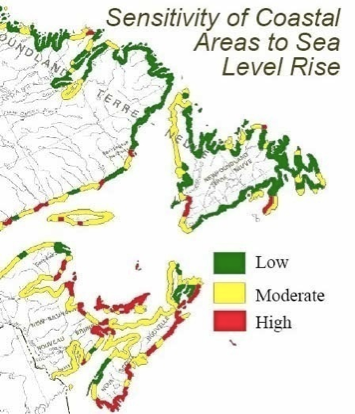
\includegraphics{s3-coastalsealevel.png}
% \centering
% \caption{Many coastal areas in all Maritime provinces are moderately to highly sensitive to the impacts of rising sea levels. (Graphic: Gary Lines)}
% \end{figure}



From Vancouver to Halifax, communities across Canada face significant risks from sea-level rise and accompanying impacts.
In the long-term, unmitigated climate change risks causing Greenland and the West Antarctic ice sheet (WAIS) to melt.
According to the IPCC: ``Near-total deglaciation would eventually lead to a sea-level rise of around 7 m and 5 m from Greenland and the WAIS, respectively, with wide-ranging consequences including a reconfiguration of coastlines worldwide and inundation of low-lying areas, particularly river deltas''.\footcite[][See: "Deglaciation of West Antarctic and Greenland ice sheets" \url{https://www.ipcc.ch/publications_and_data/ar4/wg2/en/ch19s19-3-5-2.html}]{IPCC2007}
It goes on to say that: ``Widespread deglaciation would not be reversible except on very long time-scales, if at all''.
Sea level rise on this scale would constitute an exceptionally severe social injury --- with entire countries like Bangladesh and the Netherlands massively inundated, along with low-lying regions like Florida, New York City, and many of the world's other densely populated areas.
The IPCC identifies the ``threshold for near-total deglaciation'' at 3.2--6.2°C local warming (1.9--4.6°C global warming).
This is within the range of warming projections generated by several emission scenarios studied by the IPCC, corresponding to the absence of aggressive migitation action on the part of governments.\footcite[][See: "Projected climate change an its impacts" \url{https://www.ipcc.ch/publications_and_data/ar4/syr/en/spms3.html}"]{IPCC2007}


	
	\subsubsection{Storms, droughts, and other extreme weather}



The Earth's changing climate has led to a notable rise in the number of great natural catastrophes that are driven by climate-related events over the past 25 years.\footnote{According to Munich Re, weather-related hazards can be described as a ``great natural catastrophes'' if it results in any one or a combination of the following attributes: i) number of fatalities exceeds 2,000; ii) number of homeless exceeds 200,000; iii) the country’s Gross Domestic Product (GDP) severely declines; and/or iv) the country is dependent on international aid}
Over the past 10 years, countries around the world have experienced approximately 785 natural catastrophes per year. 
During 2010 alone, a total of 950 natural catastrophes took place, nine-tenths of which were weather-related events such floods, hurricanes and storms.\footcite[][]{MunichRECatast}
Climate change is likely responsible, at least in part, for the rising frequency and severity of extreme weather events, such as floods, storms and droughts, since warmer temperatures tend to produce more violent weather patterns.\footcite[See: ][]{IPCCHurricane}
According to Environment Canada ``[f]uture warming will be accompanied by other changes, including the amount and distribution of rain, snow, and ice and the risk of extreme weather events such as heat waves, heavy rainfalls and related flooding, dry spells and/or droughts, and forest fires''.\footcite[][]{ECImpactsOfCC}



The Fourth Assessment Report of the IPCC (2007) asserts that changes in the frequency and intensity of extreme climate events will occur going into the future and will likely challenge human and natural systems to a much greater extent than natural changes in weather conditions.
These include hurricanes\footcite[][]{Knutson2004} and other extreme events including droughts, heat waves and floods.
The IPCC describes risks of extreme weather events as one of five special `reasons for concern' about climate change, along with risks to unique and threatened systems, the distribution of impacts and vulnerabilities (``those in the weakest economic position are often the most vulnerable to climate change''), aggregate impacts, and risks of large-scale singularities.\footcite[][See: "The long-term perspective" \url{https://www.ipcc.ch/publications_and_data/ar4/syr/en/spms5.html}"]{IPCC2007}
On hurricanes, the IPCC explains: ``Globally, estimates of the potential destructiveness of hurricanes show a substantial upward trend since the mid-1970s, with a trend towards longer storm duration and greater storm intensity, and the activity is strongly correlated with tropical sea surface temperature''.\footcite[][]{IPCCHurricane}
This accords with the basic science of hurricanes, which are driven by the latent heat in water vapour and gain strength from travelling over warmer water.



% \begin{figure}
% 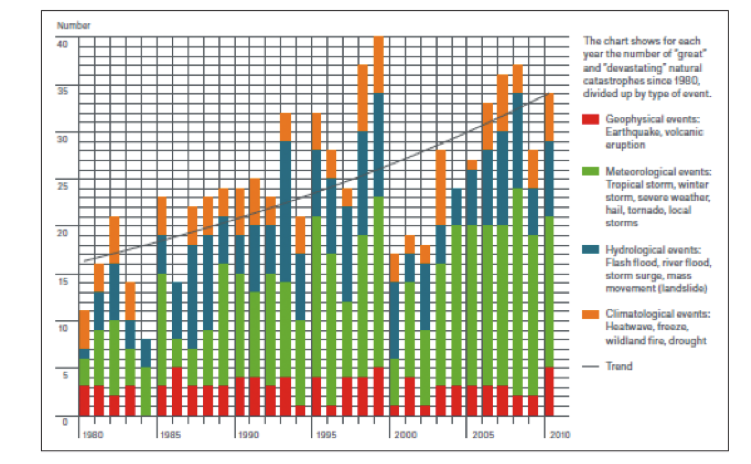
\includegraphics{s3-munich-cat.png}
% \centering
% \caption{Global trend for great natural catastrophes (as defined by Munich Re) since 1980}
% \end{figure}



In Canada, temperatures have warmed by an average of 0.24°C per decade, as indicated by data dating from the first official records of temperature conditions in 1948 through to 2010.\footcite[][p. 13]{TellingWeatherStory}
This figure represents twice the global average, with temperature rises in the far north occurring at rates three times faster. 
The average national temperature in 2010 reached 3.0°C above normal, making it the hottest year on nationwide records.\footcite[][p. 13]{TellingWeatherStory}



Precipitation levels in Canada have risen during the past half-century, with mean national levels increasing by about 12\%. 
This averages to about 20 more days of rain nation-wide compared with the 1950s. 
As climate change accelerates, and the rate of warming increases, the conditions for more volatile weather patterns become more common. 
Trends consistent with projections of climate models show increasing occurrence of extreme weather in Canada that can be traced back into the early 20th century. 
For instance, Figure ~\ref{fig:s3-canadadisasters} shows the increase in weather-related disasters in Canada over 100 years.

% \begin{figure}
% 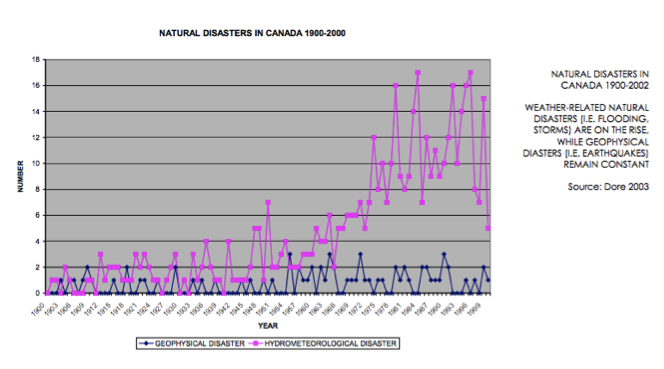
\includegraphics{s3-canadadisasters.png}
% \centering
% \caption{Source: Mohammed Dore, ``Forecasting the Conditional Probabilities of Natural Disasters in Canada as a Guide for Disaster Preparedness''}
% \label{fig:s3-canadadisasters}
% \end{figure}


By contrast, the number of geophysical disasters (earthquakes and landslides) that took place over the same time period, which has remained fairly consistent.\footcite[][p. 8]{ScanCCToronto}



With an influx of extreme weather comes mounting costs for dealing with such events. 
In the United States, private insurers determined that 2012 was the most expensive year ever in terms of disasters linked to climate change, with a total cost of \$139 billion.\footcite[][]{BlownAway}
In Canada, the NRTEE projected that total costs associated with climate change could reach between \$21 billion and \$43 billion a year by the 2050s.\footcite[][p.15]{NRTEEPrice}
The range of estimates reflects uncertainty about the extent of action taken to reduce GHG emissions as well as other economic and population growth factors. 
Similarly, a report by the Institute for Catastrophic Loss Reduction (ICLR) for the Insurance Bureau of Canada (IBC) outlines trends of insured losses from severe weather and natural catastrophes both internationally and within Canada. 
The report reveals that financial impacts have ranged from between \$10 and \$50 billion dollars a year internationally since 2002, and with levels exceeding \$100 billion in 2011.\footcite[][p. 5]{TellingWeatherStory}
Within Canada, property insurance claims resulting from severe weather-related events from 2010-2012 have cost roughly \$1B a year.
The report outlines a number of specific examples of such claims, including:
\begin{itemize}
	\item A severe wind and thunderstorm that took place on in June of 2010 in and around Leamington in Southern Ontario caused approximately \$120 million worth of insured losses to both business and residential properties.
	\item Areas in Southern Alberta experienced a similar storm that resulted in excessive damage to private and commercial properties as well as automobiles that totalled over \$500 million in losses.
\end{itemize}
As the report details, claims resulting in both severe and smaller-impact weather events represent significant property damage for consumers, with losses driven in large part from aging sewage and water infrastructure that cannot handle the new higher precipitation levels; in fact, a rise in water levels for water-related insurance claims now ``surpass[es] fire as the number one cause of home insurance losses in many parts of the country''.\footcite[][p. 7]{TellingWeatherStory}
The report also details projections running through the 2050s of extreme weather events in Canada, including hot days per year, wildfires, hail and ice storms, tornadoes, and heavy rainfall events, and includes recommendations for dealing with the expansion of insurance-related losses nationwide.


In a report for Ceres --- a  network of investors, companies, and public interest groups seeking to accelerate and expand the adoption of sustainable business practices --- Sharlene Leurig evaluated the threat of climate change to insurers.
She concluded that: ``This changing climate will profoundly alter insurers' business landscape, affecting the industry's ability to price physical perils, creating potentially vast new liabilities and threatening the performance of insurers' vast investment portfolios''.\footcite[][p. 9]{ClimateRiskInsurers}
A climate that is changing increasingly rapidly is associated with severe weather, damage to infrastructure, and soaring costs.
This corresponds with the finding of the NRTEE that ``[g]lobal mitigation leading to a low climate change future reduces costs to Canada in the long term''.\footcite[][p. 16]{NRTEEPrice}



	\subsubsection{Wildfires}
	


Increased temperatures contribute to the frequency and severity of wildfires.\footcite[][p. 33, 48, 50, 51, 53, 65 ]{IPCCar4_syr} \footcite[See also: ][]{UCSWildfire}
A 1991 study published in the \emph{Canadian Journal of Forest Research} estimated that a doubling of atmospheric \ce{CO2} would cause a 46\% increase in seasonal severity rating, with a similar increase in area burned.
A 2004 study estimated that with a doubling of \ce{CO2}, at least twice as many fires in California would ``escape'' and ``exceed initial containment limits''; that twice as large an area would be burned; and that there would be ``widespread impacts on vegetation distribution, forest condition, and carbon storage, and greatly increase the risk to property, natural resources and human life''.\footcite[][p. 169]{FriedWildfire} \footcite[See also: ][]{WesterlingWildfire}
A 2006 study of wildfire activity in the western United States found that: ``wildfire activity increased suddenly and markedly in the mid-1980s, with higher large-wildfire frequency, longer wildfire durations, and longer wildfire seasons'' and that this is ``strongly associated with increased spring and summer temperatures and an earlier spring snowmelt''.\footcite[][p. 940--943]{Westerling2006}
According to the Australian government's Climate Commission: ``Climate change has already increased the risk of extreme fire weather in some parts of Australia, especially the populous southeast.''\footcite[][p. 4]{CriticalDecade2013}



	\subsubsection{Increased risks to human health}



The impact of climate change on human health is no longer a contested issue, with major national and international organizations like the World Health Organization (WHO), Health Canada, the Centres for Disease Control and Prevention (CDC) and others recognizing both its existing impacts and its ongoing risks. 
The WHO, for example, asserts that ``the health effects of a rapidly changing climate are likely to be overwhelmingly negative, particularly in the poorest communities, which have contributed least to greenhouse gas emissions'' and acknowledges the increasingly damaging impact of an ever-warmer climate on numerous social and environmental health determinants, including clean air, water, food and shelter.\footcite[][]{WHOClimateHealth} \footcite[See also: ][]{LancetCCHealth}



The negative effects of climate change on human health can be traced back almost forty years. 
For example, a 2009 WHO report entitled \emph{Global health risks: Mortality and Burden of Disease Attributable to Selected Major Risks} found that climate change since the 1970s has contributed to diarrhoea, flood injury, malaria, undernutrition, and related disease outcomes.\footcite[][p. 44]{WHOGlobalHealthRisks}
The report explains that:
\begin{quote}
Potential risks to health include deaths from thermal extremes and weather disasters, vector-borne diseases, a higher incidence of food-related and waterborne infections, photochemical air pollutants and conflict over depleted natural resources. Climate change will have the greatest effect on health in societies with scarce resources, little technology and frail infrastructure. Only some of the many potential effects were fully quantifiable; for example, the effects of more frequent and extreme storms were excluded. Climate change was estimated to be already responsible for 3\% of diarrhoea, 3\% of malaria and 3.8\% of dengue fever deaths worldwide in 2004. Total attributable mortality was about 0.2\% of deaths in 2004; of these, 85\% were child deaths. In addition, increased temperatures hastened as many as 12 000 additional deaths; however these deaths were not included in the totals because the years of life lost by these individuals were uncertain, and possibly brief.\footcite[][p. 24]{WHOGlobalHealthRisks}
\end{quote}
The WHO also claims that global warming has been causing 140,000 deaths per year since 2004.\footcite[][]{WHOCCandHealth2012}
A more recent study commissioned by 20 governments around the world estimates that this number has grown to approximately 400,000 climate-related deaths per year.
The report finds that ``Climate change has already held back global development; it is already a significant cost to the global economy.''\footcite[][p. 16]{DARACVM}
The report also explains that: ``Continuing today's patterns of carbon-intensive energy use is estimated, together with climate 
change, to cause 6 million deaths per year by 2030, close to 700,000 of which would be due to climate change. This implies that a combined climate-carbon crisis is estimated to claim 100 million lives between now and the end of the next decade.''\footcite[][p. 17]{DARACVM}
According to a Health Canada assessment, the most significant impacts to human health driven by changes in climate are linked to temperature stress, extreme weather, rodent and water-borne diseases, ultraviolet radiation, and air pollution.\footcite[][]{HHInACC} \footnote{Notably, this is one of many climate science reports produced by Canadian civil servants and essentially `buried' by the government of Stephen Harper. Planned coast-to-coast press conferences were cancelled, the report was released without publicity, and the report is not available through the Health Canada website.}
The report describes how ``the economic costs of extreme events in this country are rapidly increasing, as is the number of people affected by natural disasters'' and that ``[s]uch events and other climate-related hazards (e.g. smog, food-, water-, vector- and rodentborne diseases) continue to pose significant short- and long-term risks to the health and well-being of Canadians and their communities''.\footcite[][p. 432]{HHInACC}



It is generally accepted that the greatest impacts of ongoing climate change will be felt by people in low-income countries, as regions with weak health or governmental infrastructure will not have the capacity to respond to consequences of climate change appropriately. 
Particularly hard hit will be children, the elderly, people with illnesses or infirmities, and people with pre-existing medical conditions. 
The WHO also claims that: ``Many of the major killers such as diarrhoeal diseases, malnutrition, malaria and dengue are highly climate-sensitive and are expected to worsen as the climate changes''.\footcite[][]{WHOCCandHealth2012}
Also, a growing body of literature is drawing attention to the incommensurate impacts of climate change on vulnerable and marginalized populations.\footcite[][p. 1693--1733]{Costello2009} \footcite[][]{WHOSocialDeterm}



Rich parts of the world are also vulnerable to health effects from climate change.
The City of New York estimates that hotter summers in the 2020s ``could cause an estimated 30 to 70 percent increase in heat-related deaths, or about 110 to 260 additional heat- related deaths per year on average in New York City compared to the baseline period for the analysis (1998–2002)''.\footcite[][p. 31]{ResilientNewYork}
According to the Australian government's Climate Commission: ``Heat causes more deaths than any other type of extreme weather event in Australia. Increasing intensity and frequency of extreme heat poses health risks for Australians and can put additional pressure on health services. Changes in temperature and rainfall may allow mosquito-borne illness like dengue fever to spread south.''\footcite[][p. 4]{CriticalDecade2013}



In Canada, the relationship of health disparities to climate change impacts and adaptation is a newly emerging area of study. 
Recent reports predict that hotter city temperatures will lead to between five and 10 additional deaths per 100,000 people per year by 2050 as well as contribute to increasing pressure on Toronto hospitals due to sickness and other heat-related conditions that could swell associated costs to between \$3 million to \$8 million annually by the 2050s.\footcite[][p. 87]{NRTEEPrice}
The NRTEE concluded that climate change ``will lead to warmer summers and poorer air quality, resulting in increased deaths and illnesses in the four cities studied — Montréal, Toronto, Calgary, and Vancouver'' and that this will impose costs on the health care system of between \$3 million and \$11 million per year by the 2050s.\footcite[][p. 16]{NRTEEPrice}



	\subsubsection{Ecosystem collapse}



Climate change is expected to have a substantial effect on ecosystems and biodiversity around the world.\footcite[][p. 1]{VulnerableSpecies}
Writing in \emph{Nature Climate Change}, a group of researchers concluded that ``without mitigation, large range contractions can be expected even amongst common and widespread species, amounting to a substantial global reduction in biodiversity and ecosystem services by the end of this century''.\footcite[][p. 1]{WarrenBiodiversity}
These ecosystems are vital to the survival and prosperity of humanity, so ecosystem damage is another important form of social injury arising from the activities of fossil fuel companies.
As emphasized by the United Nations Development Programme, the link between ecosystem integrity and prosperity is especially important for the poor: ``Climate change is already exacerbating chronic environmental threats, and ecosystem losses are constraining livelihood opportunities, especially for poor people.''\footcite[][p. 95]{UNHumanDev2013}


Salmon provide just one example of an important species that faces threats from climate change. 
The dangers climate change poses to salmon are illustrative for a number of reasons: these fish serve as an extension of the discussion relating to threats to Canadian coastal environments described above; salmon fisheries in particular are significant contributors to the global economy and to the subsistence of large segments of the world’s populations; and salmon play a critical role in the functioning of their marine ecosystems.



A report from the International Union for Conservation of Nature (IUCN) that the salmon fishing industry contributed more than \$2 billion to economies in Russia, Japan, the US and Canada and directly employed more than 35,000 people.\footcite[][p. 2]{IUCNSalmon}
Salmon are also harvested on a smaller scale, both for recreational and subsistence purposes.
Many individuals, communities and small businesses are dependent on salmon to sustain their livelihoods and to provide a significant contribution of their diet. 
Reliance on salmon fisheries as both a source of food and income is especially important to communities along Canada's Atlantic and Pacific coasts. 


In 2009, the IUCN released ``Red List of Threatened Species: More Than Just the Polar Bear'', highlighting the need to more closely study the complex risks associated with climate change to delicate ecosystems and the species that inhabit them.\footcite[][]{IUCNMorePolarBear}
The report includes a detailed discussion about the problems that increasing global temperatures will pose to the safety of the world's salmon populations. 
For instance, with respect to the role of this species in their natural environment, salmon provide food for a suite of predators and scavengers that live along the coasts of the ocean and beside the banks of streams and rivers that they traverse as part of their extensive migratory routes. 
Animals such as seals, whales, otters, bears, birds, and many invertebrates feed on salmon, many at critical stages in their own yearly feeding cycles, as a vital source of protein and fat. 
Furthermore, throughout a salmon's life cycle, it will transport essential nutrients from saltwater to freshwater areas as well as to the surrounding lands via the excretion of waste as well as through the decay of carcasses.



Increases in water temperatures concurrent with rises in global air temperatures impose a number of negative effects on salmon. 
Direct biological impacts include increased physiological stress, susceptibility and exposure to disease, and challenges and disruptions to breeding. 
These effects on the biology of salmon may potentially lead to impacts in the long-term. 
For example, because the development of salmon relies on water temperature, warmer waters could result in early migration of juvenile fish. 
Because natural patterns are timed with other important feeding phenomena such as planktonic blooms, early migrations could mean an insufficient source of food for salmon entering the oceans at a critical point in their development. 
Similarly, flows of warm freshwater can create thermal barriers to migrating salmon, requiring additional energy to navigate. 
Such barriers can also delay or even prevent spawning altogether. 
Moreover, increased winter flows can damage river beds, as well as the nests of salmon eggs dug into the sediment and gravel.



Warmer ocean temperatures have also been shown to reduce the abundance of other smaller fish into certain areas experiencing an influx of new warmer waters. 
Because the interaction of the multitude of biological factors that play a role in maintaining the balance of healthy ecosystems, scientists are hard-pressed to forecast specific predictions, let alone detail recommendations for large-scale strategies to deal with potential climate-related threats to salmon, as well as for the increasing range of at-risk species. 
Acceleration of climate change will exacerbate these difficulties, and can have profound environmental as well as economic impacts. 
The only sure means of maintaining the health of terrestrial and aquatic ecosystems is to significantly mitigate the release of greenhouse gas emissions into the atmosphere.



At the same time as they increase global temperatures, heightened \ce{CO2} concentrations in the atmosphere cause the oceans to become more acidic.
According to the IPCC, this is ``expected to have negative impacts on marine shell-forming organisms (e.g. corals) and their dependent species''.\footcite[][p. 52]{IPCCar4_syr}
The IPCC also expects ocean acidification to be part of a suite of changes that that makes it ``likely'' that ``[t]he resilience of many ecosystems'' will be ``exceeded this century''.\footcite[][p. 48]{IPCCar4_syr}
A 2010 report from the United Nations Environment Programme concluded that: ``[i]f ocean acidification continues 
disruptions to food chains and direct and indirect impacts on numerous species are considered likely with consequent risk to food security''.\footcite[][p. 8]{UNEPOceanAcid} \footcite[See also: ][]{AcidThreatFish}
The report suggests that: ``[t]he obvious solution to the potential threats posed by ocean acidification is to make rapid and substantial cuts to anthropogenic \ce{CO2} emissions to the atmosphere''.\footcite[][p. 8]{UNEPOceanAcid}



Both because of warming and because of the acidification of the world's oceans in response to rising \ce{CO2} concentrations, coral reefs are especially vulnerable to climate change.
In their fourth assessment report, the IPCC concluded that increased coral bleaching would accompany warming of 1˚C, most corals will be bleached above 1˚C, and ``widespread coral morality'' is expected above 2.5˚C.\footcite[][p.51]{IPCCar4_syr}
Significant damage to coral reefs has already been observed, including the loss of 50.7\% of initial coral cover in Australia's Great Barrier Reef.\footcite[][]{27declinecoral}
Caribbean corals are also experiencing record thermal stress, bleaching, and mortality.\footcite[][]{CaribbeanCorals}
An article in \emph{Science} explains that: ``Atmospheric carbon dioxide concentration is expected to exceed 500 parts per million... by 2050 to 2100, values that significantly exceed those of at least the past 420,000 years during which most extant marine organisms evolved''.\footcite[][p. 1737--1742]{CoralRapidCC}
It concludes that: ``[t]he result will be less diverse reef communities and carbonate reef structures that fail to be maintained''.\footcite[][p. 1737--1742]{CoralRapidCC}
As exceptionally rich ecosystems, coral reefs has an importance that goes beyond their inherent biological value.
Ecosystem services provided by coral reefs, including food, jobs, and tourism, have an estimated value of as much as \$375 billion per year.\footcite[][]{NOAACoral}



Many other species are expected to experience negative impacts from climate change.
For instance, reductions in sea ice ``will drastically shrink marine habitat for polar bears, ice-inhabiting seals, and some seabirds, pushing some species toward extinction'' while ``caribou/reindeer and other land animals are likely to be increasingly stressed as climate change alters their access to food sources, breeding grounds, and historic migration routes''.\footcite[][Executive summary, p. 10]{ACIA2004}
One 2013 study found that ``608–851 bird (6–9\%), 670–933 amphibian (11–15\%), and 47–73 coral species (6–9\%)'' are ``highly climate change vulnerable''.\footcite[][p. 1]{VulnerableSpecies}


Considerable scope exists for reducing the degree of ecosystem damage resulting from climate change by reducing future greenhouse gas pollution emissions.
The article in Nature Climate Change concludes that: ``without mitigation, $57 \pm 6\%$ of plants and $34 \pm 7\%$ of animals are likely to lose $\ge 50\%$ of their present climatic range by the 2080s. With mitigation, however, losses are reduced by 60\% if emissions peak in 2016 or 40\% if emissions peak in 2030''.\footcite[][]{WarrenBiodiversity}



	\subsubsection{Threats to First Nations groups and indigenous cultures}



Climate change threats to northern Canadian provinces, as well as the Aboriginal communities that live there, are becoming increasingly recognized. 
For example, Natural Resource Canada's recently published national assessment ``From Impacts to Adaptation: Canada in a Changing Climate 2007'' states explicitly that ``resource-dependent and Aboriginal communities are particularly vulnerable to climate changes'', and emphasizes that ``vulnerability'' to climate change risk is ``magnified in the Arctic.''\footcite[][p.3, p. 14]{ImpToAda} 
Similarly, the Arctic Council and the International Arctic Science Committee (IASC) issued a report in 2004 entitled the ``Arctic Climate Impact Assessment'' that aimed  to synthesize knowledge on climate variability and to assess and predict the impact of climate change on arctic regions and communities going into the future.\footcite[][]{ACIA2004}
The report contains contributions from over 300 scientists, professionals, and Aboriginal community leaders and reveals that future climate change could be devastating for numerous Inuit communities.
These findings are supported by a more recent study conducted by researchers from McGill University that focused on two separate Inuit communities.\footcite[][]{CCInuitCommunities}
The study identifies that ``climatic conditions which currently pose risks are expected to be negatively affected by future climate change'' and explains that ``young Inuit and those without access to economic resources, in particular, are vulnerable''.\footcite[][p. 45, p. 54]{CCInuitCommunities}



According to a 2009 article in \emph{Global Environmental Change}, ``health inequality [in relation to climate change] is
particularly pronounced among Aboriginal Canadians''.\footcite[][p. 1]{VulAborig2009}
While climate change in general `` has been identified as potentially the biggest health threat of the 21st century'', the article goes on to explain that ``[t]he existing burden of ill-health increases the sensitivity of Indigenous peoples to the adverse impacts of climate change, which combined with a proportionally higher dependence of many Indigenous livelihoods on the environment, spiritual and cultural ties to the land, demographic trends, and experience of marginalization, makes Indigenous peoples particularly vulnerable''.\footcite[][p. 1]{VulAborig2009}



	\subsubsection{Threats to the infrastructure of cities, including Toronto}



More than half the world's population live in cities and urban areas. 
As a first step towards addressing climate change, many cities have conducted assessments of their GHG emissions. 
In Canada, over 200 municipalities are taking part in the Partners for Climate Protection  program, which is the Canadian component of International Council for Local Environmental Initiatives's Cities for Climate Protection network.\footnote{See: \url{http://www.icleicanada.org/programs/mitigation/pcp}}
The Province of Ontario and the City of Toronto are among those actively implementing numerous plans and initiatives to reduce GHG pollution. 
The first attempt on behalf of the City to assess GHG levels came in 2004.\footcite[][p. IV]{GHGPollutionToronto}
Follow-up reports detailing strategies for reducing emissions were published soon after.\footcite[][]{CCAHealthEquity}
Additionally, there is a growing body of literature that examines current trends and anticipated affects of climate change to Toronto and surrounding areas.\footcite[][]{TorontoEnvOff2007} \footcite[][]{TorontoAheadStorm} \footcite[][]{ScanCCToronto} \footcite[][]{AdaptPrioritiesCanada} \footcite[][]{MacLeodAdaptation}



The City of New York projects that --- because of rising sea levels and ocean temperatures --- by 2050 ``a storm like [Hurricane Sandy could cause an estimated \$90 billion in losses (in current dollars) --- almost five times as much''.\footcite[][Foreward, p. 2]{ResilientNewYork}



It is now generally recognized that impacts of climate change are already being felt in Toronto and the GTA.
Toronto has experienced extreme heat, floods, droughts, new insect pests, new vector-borne diseases and other problems worsened by climate change.\footcite[][]{TorontoAheadStorm}
In terms of fluctuations to regular weather patterns, Toronto has seen an average temperature increase of 2.7°C since the late 1800s.\footcite[][p. 5]{ScanCCToronto}



Record high temperatures, accompanied by smoggier skies, have also been recorded in recent summer seasons. 
For instance, 2005 saw the warmest June on record: 37 days had a maximum temperature greater than 30°C (more than double the average from 1971-2000); humidex values exceeded 35 more than 44 times; and 48 smog days were declared, the highest number on record.\footcite[][p. iii, p. 7]{ScanCCToronto}
While precipitation patterns have not undergone such drastic changes, it has been predicted that precipitation will likely arrive during heavy rainfall events. \footcite[][p. 6]{ScanCCToronto}
For instance, snowfall is expected to decrease and rainfall will increase in its stead, accompanied by an influx of freezing rain episodes.\footcite[][p. 8]{TorontoAheadStorm}
More ice-storms are also expected.\footcite[][]{FreezingRain2007}
More freeze-thaw cycles in the city are also projected, which take a heavy toll on roads as well as urban green spaces.\footcite[][p. 8]{TorontoAheadStorm}



\textbf{Increased financial burdens on the city}



High density cities such as Toronto are particularly susceptible to damage caused by extreme weather or natural disasters. 
Extreme weather events occurring as a consequence of climate change can also be extremely costly for municipalities that have to deal with the consequences and clean-up. 
For example, the intense storm that took place in the city on August 19, 2005 caused millions of dollars of damage. 
This storm's heavy rainfall washed out a part of Finch Avenue, and caused flash flooding and widespread damage across the city. 
Parks and Recreation spent \$12.5 million restoring damaged trees and urban parks. 
\$600,000 was spent by Urban Forestry Services to clear fallen trees.\footcite[][p. iii]{ScanCCToronto}
Likewise, Transportation Services spent close to \$5 million repairing Finch Avenue. 
The total damage, including public and private property, was estimated at approximately \$400 -- \$500 million --- the most expensive storm in Toronto's history.\footcite[][p. 11]{TorontoAheadStorm}



More frequent storms and severe weather will likely continue to cause damage to city infrastructure and put strain on city resources. 
Indeed, the floods, storms, droughts and other weather-related phenomena that already occur annually in Canada can cost hundreds of millions of dollars.\footcite[][p. 11]{HHInACC}
Furthermore, recent events such as Hurricane Sandy have revealed that even developed countries can be devastated by extreme weather events that are difficult to prepare for and which can be unprecedented in terms of strength and geographic scope.   



\textbf{Increased health risks to vulnerable populations}



While severe storms and extreme weather can be very costly, the longer-term  impacts of climate change will have an adverse affect on the city and its residents in ways that ``[go] well beyond the reported monetary costs''.\footcite[][p. 19]{CCAHealthEquity}
It is widely documented that certain populations in a particular city are more vulnerable to the adverse affects of climate change than others.\footcite[][]{EbiHealthJustice} \footcite[][]{HotWeatherResponse2006} \footcite[][p. 1153--1163]{MarmotHealthOutcomes} \footcite[][]{ReducingHealthDisparities}
`Vulnerability' in this sense can be defined as ``the degree to which individuals and systems are susceptible to or unable to cope with the adverse effects of climate change''.\footcite[][p. 6]{CCAHealthEquity}
Determinants of health, such as income and social status, education and literacy, social and physical environments, or genetics, etc., can be used to assess a population's vulnerability to the various impacts of climate change. 
For example, severe storm events can affect physical environments by causing extensive property damage; challenges linked with income and social status can be reinforced as those with inadequate employment or insufficient funds could have more difficulty acquiring financial resources to repair property, deal with displacement, or finance interim accommodation. 
Populations that are particularly vulnerable to climate change impacts in the City of Toronto, include infants and babies, women, the elderly, those with preexisting or underlying conditions, First Nations, those whose livelihood is reliant on natural resources, and those with low social and economic standings.\footcite{CCAHealthEquity} \footcite[][]{HHInACC} \footcite[][]{HealthCanadaPreparingImpacts}



The current and forecasted future makeup of the City of Toronto is one that is both highly diverse and increasingly expanding; indeed, the population of the Greater Toronto Area is estimated to reach 9.2 million by 2036.\footcite[][]{DemoProjections2012}
Toronto's swelling population encompasses a number of the vulnerable populations identified above. 
For instance, according to Statistics Canada, the First Nations population of the city grew 20\% from 2001, reaching a total of 13,605 people as of 2006.\footcite[][]{2006TorontoProfile}
This figure represents over 0.5\% of the total population in the City, and 43\% of the First Nations population in the Greater Toronto Area (GTA). 
Moreover, Statistics Canada reports that the City of Toronto was home to over 350,000 seniors in 2006.
This number constitutes 14\% of the City’s population, and 53\% of all seniors living in the GTA. 
The city's Social Development, Finance and Administrative Division forecasts that seniors will make up 17\% of the City of Toronto population by 2031.\footcite[][p. 5]{SeniorsDemographicSnapshot}
Finally, an increasing number of Torontonians are low-income.
For instance, in 2005 there were 134,247 family households and 165,156 persons not living in family households that reported before-tax income levels below Statistics Canada's Low Income Cut-off.\footcite[][p. 5]{LowIncomeProfile}
The size of the low-income population recorded in 2005 was greater than in the early 1990s, and represents almost double the size as in the rest of the GTA.\footcite[][p. 6]{LowIncomeProfile}



The literature on health equity in a Canadian context shows a direct relationship between health and income.\footcite[][]{HotWeatherResponse2006} \footcite[][]{PovertyMakingSick} \footcite[][]{PovertyInequalityHealth}
People living in poor areas in Toronto experience increased risk factors for illness, higher occurrence of disease, and early mortality than people who reside in more affluent areas.
Such risks will very likely be aggravated by the impacts of climate change on the city.
A Waterloo-based study exploring the connection between effects of climate change and the homeless population found that exposure to extreme weather was high for this segment of the population; furthermore, exposure exacerbated pre-existing illnesses such as drug and alcohol addictions, mental illness, cardiovascular and respiratory conditions, as well as feelings of isolation and increased stress.\footcite[][]{HomelessnessWaterloo}



A more comprehensive examination of the various ways that the City of Toronto will suffer social, economic, and environmental injury as a direct result of climate change can be found in the 2009 Clean Air Partnership Report ``Climate Change Adaptation and Health Equity''.\footcite[][]{CCAHealthEquity}
It includes details about the affect of impacts on Toronto's water supply and water quality, energy sources, transportation sector and services, buildings and infrastructure, urban ecosystem, tourism, and economy.  



	\subsubsection{Abrupt and non-linear adverse climate impacts}



The Earth's climate system includes some powerful positive feedback mechanisms capable of multiplying the climate-altering effect of greenhouse gases.
These include the way in which melting ice decreases the planet's albedo (reflectiveness), causing more of the sun's energy to be directed toward increasing temperatures.
Other feedback mechanisms include the release of methane --- a powerful greenhouse gas --- from melting permafrost and subsea methane clathrate deposits.
Abrupt methane release has been associated with past instances of abrupt global warming, such as during the Paleocene–Eocene Thermal Maximum 55 million years ago, and several of these instances were accompanied by major global extinction events both on land and in the oceans.\footcite[See: ][]{Hansen2010}
According to NASA:
\begin{quote}
Over hundreds of millennia, Arctic permafrost soils have accumulated vast stores of organic carbon --- an estimated 1,400 to 1,850 petagrams of it (a petagram is 2.2 trillion pounds, or 1 billion metric tons). That's about half of all the estimated organic carbon stored in Earth's soils. In comparison, about 350 petagrams of carbon have been emitted from all fossil-fuel combustion and human activities since 1850. Most of this carbon is located in thaw-vulnerable topsoils within 10 feet (3 meters) of the surface.
\end{quote}
NASA also explains that ``Permafrost soils are warming even faster than Arctic air temperatures ... 1.5 to 2.5 degrees Celsius in just the past 30 years'' and that this warming ``threatens to mobilize these organic carbon reservoirs and release them into the atmosphere as carbon dioxide and methane, upsetting the Arctic's carbon balance and greatly exacerbating global warming''.\footcite[][]{SleepingGiant}


Several potentially dangerous `tipping points' have been identified by scientists, including the danger that the themohaline circulation which produces Europe's relatively warm climate relative to its latitude may be disrupted, though this is now considered unlikely, at least within the next century.\footcite[][]{IPCCThermohaline}
Writing in \emph{Nature} in 2009, Johan Rockstrom et al. explain that:
\begin{quote}
We propose that human changes to atmospheric \ce{CO2} concentrations should not exceed 350 parts per million by volume, and that radiative forcing should not exceed 1 watt per square metre above pre-industrial levels. Transgressing these boundaries will increase the risk of irreversible climate change, such as the loss of major ice sheets, accelerated sea level rise and abrupt shifts in forest and agricultural systems. Current \ce{CO2} concentration stands at 387 p.p.m.v. and the change in radiative forcing is 1.5 W $m^{−2}$ 
\end{quote}
In their Fourth Assessment Report, the IPCC explains that ``[a]nthropogenic warming could lead to some impacts that are abrupt or irreversible'', including in the form of ``metres of sea level rise'', ``significant extinctions'' (40 to 70\% of species assessed if warming exceeds 3.5˚C), and ``[c]hanges in terrestrial and ocean \ce{CO2} uptake [that] may feed back on the climate system''.\footcite[][p. 53]{IPCCar4_syr}




The climate system has experienced dramatic changes in the past, such as the Permian–Triassic extinction event.
This event, which took place 252 million years ago, saw 96\% of marine species and 70\% of terrestrial species become extinct, and took as long as 10 million years to recover from.\footcite[][p. 759--765]{PTRecovery}
Possible caused by volcanism, this event involved ``global warming by 6˚C and huge input of light carbon into the ocean-atmosphere system'' and ``an ever-worsening positive-feedback loop, the `runaway greenhouse'.''\footcite[][p. 358]{EndPermian}
It is possible that human GHG pollution on a significant scale could induce massive additional GHG release as permafrost and clathrates melt, and as forests dry out and burn.
A severely amplified anthropogenic greenhouse effect could pose a significant danger to human civilization and many forms of life on Earth.



The planet Venus may have experienced a `runaway' climate change scenario.
Beginning in a state where liquid water existed on its surface, as the result of the sun growing brighter over long periods of time Venus experienced an accumulation of water vapour and \ce{CO2} in its atmosphere.\footcite[][]{VenusRunaway}
Now the surface of the planet has an average temperature of 462˚C.
NASA climatologist James Hansen has suggested that the Earth could experience a runaway greenhouse effect and adopt a climate like that of Venus if fossil-fuel use continues until reserves are exhausted.\footcite[][p. 22-23]{HansenVenusThreat}



	\subsubsection{Security implications}
	
	
	
A number of major analyses have been focused on the likely global security implications of climate change.
In 2008, a National Intelligence Assessment was assembled by 16 U.S. intelligence agencies.
While the report is classified, the chairman stated publicly that climate change could disrupt US access to raw materials, create millions of refugees, and cause water shortages and damage from melting permafrost.\footcite[][]{Craven}
A 2003 report commissioned by the Pentagon considered some of the more dramatic possible warming scenarios and concluded that:
\begin{quote}
In short, while the US itself will be relatively better off and with more adaptive capacity, it will find itself in a world where Europe will be struggling internally, large number so [sic] refugees washing up on its shores and Asia in serious crisis over food and water. Disruption and conflict will be endemic features of life.\footcite[][p. 22]{AbruptCCScenario}
\end{quote}
It also argues that: ``with inadequate preparation, the result [of abrupt climate change] could be a significant drop in the human carrying capacity of the Earth’s environment''.\footcite[][p. 1]{AbruptCCScenario}
A report prepared for the Center for Naval Analysis --- produced by a ``blue-ribbon panel of retired admirals and generals from the Army, Navy, Air Force, and Marines'' --- calls climate change ``potentially devastating''.\footcite[][p. 3]{NationalSecurityCC}
A joint report from the Center for Strategic and International Studies and the Center for a New American Security describes how current projections from climate models are ``too conservative'' and that ``at higher ranges of the [warming] spectrum, chaos awaits''.\footcite[][p. 78]{AgeOfConsequences}
The report also highlights the need for urgent action to reduce emissions: ``An effective response to the challenge of global warming cannot be spread out across the next century, but rather must be set in place in the next decade, in order to have any chance to meaningfully alter the slope of the curves one sees in the IPCC report''.\footcite[][p. 78]{AgeOfConsequences}



In 2012, the U.S. National Academy of Sciences published a report on: ``Climate and Social Stress: Implications for Security Analysis''.\footcite[][]{SocialStress}
The report concludes that:
\begin{quote}
Anthropogenic climate change can reasonably be expected to increase the frequency and intensity of a variety of potentially disruptive environmental events— slowly at first, but then more quickly. Some of this change is already discernible. Many of these events will stress communities, societies, governments, and the globally integrated systems that support human well-being.\footcite[][p. S-2]{SocialStress}
\end{quote}
And that:
\begin{quote}
It is prudent to expect that over the course of a decade some climate events—including single events, conjunctions of events occurring simultaneously or in sequence in particular locations, and events affecting globally integrated systems that provide for human well-being—will produce consequences that exceed the capacity of the affected societies or global systems to manage and that have global security implications serious enough to compel international response. It is also prudent to expect that such consequences will become more common further in the future.\footcite[][p. S-4]{SocialStress}
\end{quote}
All told, the report describes in great detail the ways in which climate change is a national security issue for the United States, as well as a threat to international peace and security.


In March 2013, Admiral Samuel J. Locklear III --- the chief of U.S. naval forces in the Pacific --- argued that climate change ``is probably the most likely thing that is going to happen... that will cripple the security environment, probably more likely than the other scenarios we all often talk about''.\footcite[][]{PacificChiefWorry}



In 2012, officials from the Canadian Security and Intelligence Service and Department of National Defence attended a briefing on the security risks posed by climate change.\footcite[][]{CCSecurityBriefing}
The presentation --- which has been declassified for release through access to information legislation --- described climate change impacts including extreme weather events, impacts on coastal cities, damage to food security, and loss of biodiversity.



	\subsection{The harm caused is inherent to the primary business of fossil fuel companies}



All the social injuries described above are imposed on innocent parties by fossil fuel companies in the course of their fundamental business activity of digging up coal, oil, and gas.
These harms are inseparable from the continuation and expansion of these core business activities.
As a result, shareholder voice is not an effective strategy for mitigating these harms. 
The value of these companies also reflects the assumption that these reserves will be extracted and burned.
The University of Toronto's investments in these companies increase the amount of harm that will arise as a result of climate change.



Divestment is the only way for the University of Toronto to avoid contributing financially to the fossil fuel industry, and by extension, to the socially injurious impacts delineated above.
Besides divestment, another approach to socially responsible investment is to try to alter a firm’s behaviour by applying pressure through shareholder voice. 
However, the harmful activities (extracting and selling fossil fuels) are inherent to the primary business of fossil fuels companies in which the university is invested.  
In this sense, investments in fossil fuel companies closely parallel investments in tobacco companies; in both cases, the problem is the primary product being produced by the industry.



For example, Shell Canada lists its business activities as follows: ``Shell Canada's Upstream businesses explore for and extract natural gas, and market and trade natural gas and power. Our Downstream business refines, supplies, trades and ships crude oil worldwide and manufactures and markets a range of products, including fuels, lubricants, bitumen and liquified petroleum gas (LPG) for home, transport and industrial use.''\footcite[][]{ShellAtAGlance}
ExxonMobil describes its upstream and downstream activities similarly.\footcite[][]{ExxonWhatWeDo}



Given the centrality of oil and natural gas extraction, as well as the refinement and sale of these resources to the business models of these companies, shareholder voice would not be an effective method to address social injury since the companies could not abandon the socially injurious activity without dissolving their existing business models.  
Moreover, the market value of these companies reflects an assumption that their reserves will be extracted and burned.  
Therefore, it would be unreasonable for the University of Toronto to expect to be able to alter the socially injurious activities of these companies while holding onto its investments in the fossil fuel industry.  
Thus, divestment is the only appropriate response for the University of Toronto to adopt in order to dissolve any financial complicity in the fossil fuels industry’s socially injurious activities.  



	\subsection{The business activities of these companies frustrate the enforcement of the rules of domestic and international law intended to protect individuals against deprivation of health, safety, and basic freedoms}
	\label{sec:FrustrateLaw}



The socially injurious activities of fossil fuel companies frustrate the enforcement of rules of domestic and international law intended to protect individuals against deprivation of health, safety and basic freedoms.  
This includes the violation of specific domestic and international statutes, the violation of common law duties such as through the creation of nuisance, and the frustration of international diplomatic efforts to address climate change.



	\subsubsection{Canadian domestic law}



At the highest level, the activities of fossil fuel companies risk undermining the \emph{Canadian Charter of Rights and Freedoms}.  
Section 7 states: ``the right to life, liberty and security of the person and the right not to be deprived thereof except in accordance with the principles of fundamental justice''.\footcite[][]{CharterRF}
Arguably, the harms associated with climate change could become so substantial as to deprive people of these rights.
In particular, that could be the case for particularly vulnerable populations and communities within Canada, such as small northern settlements.
Settlements built on permafrost could become too dangerous to inhabit, while those dependent on ice roads for supplies could become too isolated to be economically viable.
Further, if the sea level rise projections discussed in \nameref{sec:inundationcoastal} prove justified, the security of the person and lives of many people across Canada could be threatened.



The activities of the fossil fuels industry in Canada also violate the constitutional and treaty rights of Canada's First Nations.
These violations arise both from the specific impact of fossil fuel development projects --- such as the oil sands --- and from the inevitable consequences of burning fossil fuels.
Rights that are being violated include the right to consultation and accommodation; the right to fish, hunt, and trap; and the aboriginal rights affirmed in Canada's constitution.
Keepers of the Athabasca member Vivienne Beisel explains how the oil sands development has violated Treaty 8 and the constitution:
\begin{quote}
``The cumulative impacts of oil sands development has all but destroyed the traditional livelihood of First Nations in northern Athabasca watershed.  The law is clear that First Nations must be consulted whenever the province contemplates action that may negatively affect Aboriginal and treaty rights... The province has continued to issue approvals for new developments without obtaining their consent or consulting with First Nations in a meaningful and substantial way. This is in direct breach of Treaty 8 First Nations' treaty-protected Aboriginal rights to livelihood, and thus a violation of s.35(1) of the Constitution''.
\end{quote}
In June 2013, the Lac La Biche-area Cree won a case at the Court of Appeal of Alberta allowing them to proceed with a lawsuit against the Canadian federal government and the Government of Alberta.
The Cree allege that the cumulative impacts of 300 operating oil sands projects impact their rights to hunt and fish under Treaty 6.\footcite[][]{BandWinsTreatyRights}
560,000 barrels of out per day are being extracted from the territory in question - 30\% of the total output from the oil sands.
Future projects that have been announced would increase that total to 1.6 million barrels per day.



The impact of climate change is being felt disproportionately in Canada's arctic.
This makes it a particular threat to the way of life of the Inuit.
Melting permafrost, the loss of summer sea ice, and impacts on marine mammal populations all threaten to substantially affect their way of life, culture, and economic subsistence.
Canadian Inuit activist and former International Chair for Inuit Circumpolar Council discusses these issues at length in her book \emph{The Right to be Cold}.\footcite[][]{RightToBeCold}



In addition, numerous pieces of Canadian environmental legislation explicitly recognize and seek to protect the right to a healthful environment.
The 1993 \emph{Ontario Environmental Bill of Rights} recognizes the ``inherent value of the natural environment'' and states that ``the people of Ontario have the right to a healthful environment'' and ``have as a common goal the protection, conservation and restoration of the natural environment for the benefit of present and future generations''.\footcite[][]{OntBillRights}
The purposes of the act are:
\begin{enumerate}
	\item to protect, conserve and, where reasonable, restore the integrity of the environment by the means provided in this Act;
	\item to provide sustainability of the environment by the means provided in this Act; and
	\item to protect the right to a healthful environment by the means provided in this Act.
\end{enumerate}
The above purposes include the following:
\begin{enumerate}
	\item The prevention, reduction and elimination of the use, generation and release of pollutants that are an unreasonable threat to the integrity of the environment.
	\item The protection and conservation of biological, ecological and genetic diversity.
	\item The protection and conservation of natural resources, including plant life, animal life and ecological systems.
	\item The encouragement of the wise management of our natural resources, including plant life, animal life and ecological systems.
	\item The identification, protection and conservation of ecologically sensitive areas or processes. (2). 
\end{enumerate}
Through numerous mechanisms described in this brief, the activities of fossil fuel companies undermine the integrity and sustainability of the environment, along with the right of the population of Ontario to a healthful environment.
GHG pollution poses an unreasonable threat to the integrity of the environment, while threatening biodiversity and the ability of Ontario to manage natural resources wisely and protect sensitive areas.



Environmental laws in Canada's provinces recognize and seek to protect the same right to a healthy environment.  
For example, the \emph{Yukon Environment Act} states that: ``The people of the Yukon have the right to a healthful natural environment''.\footcite[][p. 14]{YukonEnvAct}
Among its objectives, the act also seeks: ``to ensure the maintenance of essential ecological processes and the preservation of biological diversity'', ``to ensure comprehensive and integrated consideration of environmental and socioeconomic effects in public policy making in the Yukon'', and ``to fully use the knowledge and experience of Yukon residents in formulating public policy on the environment''.\footcite[][p. 13]{YukonEnvAct}
Because of the general failure to deal with climate change effectively in Canada, these objectives are currently being frustrated.
Similarly, the Northwest Territories \emph{Environmental Rights Act} recognizes that ``the people of the Northwest Territories have the right to a healthy environment and a right to protect the integrity, biological diversity and productivity of the ecosystems in the Northwest Territories'' and establishes the means by which individuals can act to protect the environment from harm.\footcite[][]{NWTEnvRightsAct}
By pursuing the extraction of fossil fuels, the companies in question undermine the right to a healthy environment that this acts endeavours to protect. 
Finally, Quebec's \emph{Environmental Quality Act} states that: ``[e]very person has a right to a healthy environment and to its protection, and to the protection of the living species inhabiting it'' and that: ``A judge of the Superior Court may grant an injunction to prohibit any act or operation which interferes or might interfere with the exercise of [these] right[s]''.\footcite[][]{QuebecEQA}



In several instances, Canadian courts have recognized the seriousness of climate change in their decisions.

\begin{vcom}
Find as many examples as possible for the paragraph above
\end{vcom}


Over and above violations of specific pieces of legislation, climate change represents a massive example of `nuisance' as defined in Canadian tort law.
Under the common law in Canada ``a landowner's right to use and enjoy his property doesn't give him the right to engage in activities that interfere with the rights of neighbours to use and enjoy their own properties''.\footcite[][]{NuisancesInsider}
That is to say, the fact that fossil fuel companies own the land and mineral rights in the areas where they are operating does not mean they have the right to impose extreme weather, rising sea levels, and other well-understood climate change harms on other landowners across Canada.
This principle is also incorporated into the bylaws of many Canadian jurisdictions.
For instance, the town of Musgrave, Nova Scotia has a nuisance bylaw stating: ``No person shall cause, suffer or allow to be discharged or emitted from any fuel burning equipment, internal combustion engine, vehicle or outside open fire any smoke, dust, fly-ash, soot or fumes or other solid or gaseous product or combustion to an extent which is detrimental to the property of any other person''.\footcite[][]{NuisancesInsider}
Nuisances are also regulated under provincial and territorial law.



		\subsubsection{U.S. domestic law}



In a report prepared for the U.S. Congressional Research Service, Robert Meltz discusses many of the legal issues associated with climate change.\footcite[][]{ExistingLaw}
This includes questions about the power of various bodies to impose limits on GHG pollution.
It also includes issues of liability for harm caused by climate change, including through water shortages, sea level rise, and extreme precipitation.
While the answers to these questions are not clear in the United States, and barriers to litigation exist, it is conceivable that as the severity of climate change increases and the harms being imposed by GHG pollution become more evident, courts will show a greater willingness to recognize climate change as an issue where victims can seek recompense for damage and in which the unlimited appetite of polluters to make free use of the atmosphere may be curbed.



In 2007, the U.S. Supreme Court decided ``Massachusetts v. Environmental Protection Agency'' --- a suit brought by twelve states and several cities against the Environmental Protection Agency (EPA).\footcite[][]{MassVEPA}
The court held that the Clean Air Act grants the EPA the authority to regulate tailpipe emissions of GHGs, and required the EPA to review its rationale for not regulating \ce{CO2} and other GHG emissions:
\begin{quote}
Under the clear terms of the Clean Air Act, EPA can avoid taking further action only if it determines that greenhouse gases do not contribute to climate change or if it provides some reasonable explanation as to why it cannot or will not exercise its discretion to determine whether they do.\footcite[][p. 30]{MassVEPA}
\end{quote}
The court found that the failure of the EPA to regulate GHG emissions under the CAA violated the law's ``clear statutory command''.\footcite[See: ][]{EPAhaspower}
In 2009, the EPA responded by deciding that six GHGs are indeed a danger to the environment and human health.\footcite[][]{GreenFigleaf}



Later in 2007, the U.S. Ninth Circuit Court of Appeals ruled on ``Center for Biological Diversity vs. National Highway Traffic Safety Administration''.\footcite[][]{9thcircuitHighway}
In this suit, the Center for Biological Diversity headed an alliance included 11 states, two cities, and four environmental groups calling for rigorous analysis of greenhouse gas emissions in the National Environmental Policy Act (NEPA) process. 
Specifically, this alliance challenged a rule broadcast by the National Highway Traffic Safety Administration (NHTSA) entitled: ``Average Fuel Economy Standards for Light Trucks, Model Years 2008-2011''.
This rule set corporate average fuel economy (CAFE) standards in accordance with the Energy Policy and Conservation Act (EPCA) and prior to the passage of a new energy bill.  
In this decision, the court overturned the government's lenient fuel economy standards for pick-up trucks and sport utility vehicles on the basis of a number of violations, including failure to adequately consider the greenhouse gas implications of the standards in the NEPA analysis and ``failure to monetize the value of carbon emissions''.
The court found that the ``impact of greenhouse gas emissions on climate change is precisely the kind of cumulative impact analysis that NEPA requires agencies to conduct''.
The Center for Climate and Energy solutions explains that ``[t]he court also discredited contrary precedent by stating more is now known about climate change'', holding that the 2007 ruling ``Massachusetts v. Environmental Protection Agency'' is ``more relevant than past cases where climate change science was allowed to be ignored''.\footcite[][]{NEPACases}
The New York Times described the ruling as ``a major setback for both the auto industry and the White House at a time of growing public concern over the rising price of gasoline and the issue of climate change''.\footcite[][]{CourtRejectsTruckStandards}



		\subsubsection{Domestic law in other jurisdictions}
		
		
		
A limited recognition of the seriousness of climate change can be found in some legal decisions from the United Kingdom.
For instance, in 2008 jurors decided that damage caused by activists to the Kingsnorth power station in Kent was justifiable in light of the amount of environmental damage being done by the power plant.\footcite[][]{JuryDecides}
During the trial, the jurors heard testimony from NASA climatologist James Hansen.


When it added articles 71--74 to its constitution in 2008, Ecuador became the first nation to grant the environment the inalienable right to exist, persist, and be respected.
For instance, article 73 holds that: ``The State shall apply preventive and restrictive measures on activities that might lead to the extinction of species, the destruction of ecosystems and the permanent alteration of natural cycles''.\footcite[][]{EcuadorConstitution}
Following this example, Bolivia amended its constitution in 2011 with the Rights of Mother Earth Act (articles 56-60).\footcite[][p. 28--29]{BoliviaConstitution} \footcite[][]{BoliviaGives}



The domestic law of several other states criminalizes ``ecocide'' --- a phenomenon defined by Polly Higgins as: ``The extensive damage to, destruction of or loss of ecosystem(s) of a given territory, whether by human agency or by other causes, to such an extent that peaceful enjoyment by the inhabitants of that territory has been or will be severely diminished''.\footcite[][]{EradicatingEcocide}
Article 342 of the \emph{Penal Code} of Vietnam concerns ``crimes against mankind'' and states that:
\begin{quote}
Those who, in time of war, give the order for or directly undertake the murder of civilians, wounded persons, prisoners of war, the looting of property, the destruction of population quarters, the use of banned war means or methods, and/or commit other acts in serious violation of international laws or international treaties which Vietnam has signed or acceded to, shall be sentenced to between ten years and twenty years of imprisonment, life imprisonment or capital punishment.\footcite[][]{VietnamPenalCode}
\end{quote}
Article 394 of the \emph{Criminal Code of the Republic of Armenia} similarly prohibits ecocide, as does the \emph{Criminal Code} of Belarus, the \emph{Criminal Code} of Moldova, the \emph{Criminal Code} of Ukraine, and the \emph{Criminal Code} of Georgia.\footcite[][]{ArmeniaCriminalCode} \footcite[][]{ICRConBelarusCC} \footcite[][]{MoldovaCriminal} \footcite[][]{UkraineCriminal} \footcite[][]{GeorgiaCriminal}



		\subsubsection{International law}



The activities of the fossil fuels companies in which the University of Toronto invests also frustrate international law.  
First, the \emph{Universal Declaration of Human Rights} states that ``Everyone has the right to life, liberty and security of person''.\footcite[][]{UniversalDeclarationOfHumanRights}
The right to life is a precondition to all other fundamental human rights.  
The activities of companies in the fossil fuels industry threaten the rights to life and security of the person through mechanisms including the increased frequency and severity of extreme weather, increased occurrence of infectious disease, and loss of  agricultural productivity.
In addition, the 1989 \emph{Hague Declaration on the Environment}, to which Canada is a signatory, makes the link between the right to life and the harmful change effects of climate change explicit: ``The right to live is the right from which all other rights stem. Guaranteeing this right is the paramount duty of those in charge of all States throughout the world.  Today, the very conditions of life on our planet are threatened by the severe attacks to which the earth's atmosphere is subjected''.\footcite[][]{HagueDeclarationOnTheEnvironment}   
In signing onto this declaration, Canada recognized the reality of the threat to human life posed by climate change and pledged to take measures to address that threat.
The determination of fossil fuel companies to dig up and burn their entire reserves of coal, oil, and gas directly frustrates these international laws.
If fossil fuel companies are able to continue to operate under business-as-usual conditions and execute their business plans, the world will experience far more than 2˚C of climate change, with severe impacts on people everywhere.



Fossil fuel companies have repeatedly also frustrated the enforcement of the International Labour Organization's \emph{Indigenous and Tribal Peoples Convention, 1989}.\footcite[][]{ILOConv169}
This convention requires that indigenous populations be ``consulted on issues that affect them'' and that they be able to ``engage in free, prior and informed participation in policy and development processes that affect them''.
In many parts of the world, oil, gas, and coal extraction have taken place without such consultation, or even in the face of active and energetic opposition from indigenous groups.
The activities of Shell in the Niger Delta --- described more comprehensively in \nameref{sec:Shell} --- are an especially notable and egregious example.



The political influence of fossil fuel corporations in Canada has pushed the federal government to adopt obstructionist tactics at international climate change negotiations.
For example, Canada has repeatedly been `awarded' satirical `Fossil of the Year' award for obstructing negotiations at the Conferences of the Parties (COP) of the United Nations Framework Convention on Climate Change (UNFCCC).\footcite[][]{DurbanFossil} \footcite[See also: ][]{SimpsonBlustering}
At the Copenhagen COP in 2009, a coalition of environmental groups declared Canada ``the absolute worst country at the talks''.\footcite[][]{CBCFossil}



The activities of fossil fuel companies are also at odds with the fundamental objective of the UNFCCC, which was ratified by Canada and which entered into force on March 21st 1994.
The UNFCCC affirms the intention of signatories to achieve ``stabilization of greenhouse gas concentrations in the atmosphere at a level that would prevent dangerous anthropogenic interference with the climate system''.\footcite[][p. 4]{UNFCCC}
Countries including Canada have since adopted a threshold of 2˚C of global temperature increase above pre-industrial levels as constituting `dangerous' climate change.
Canada's behaviour to date --- and the behaviour of fossil fuel companies --- has not been consistent with achieving this objective.
Achieving this objective requires that most of the reserves of fossil fuel companies be left unburned underground.
It also requires the abandonment of projects intended to extract unconventional reserves of fossil fuels, through activities including oil and gas drilling in the arctic, exploitation of the oil sands, and extraction of previously inaccessible oil and gas reserves through hydraulic fracturing.
Rather than curtailing such activities, the Government of Canada has worked intently to reduce the environmental oversight to which the oil sands are subjected, while aggressively pushing pipelines and other projects to increase the export capacity of the oil sands.



Despite ratifying the Kyoto Protocol in 2002, the Government of Canada never developed a serious plan to achieve the target it selected for itself: a reduction in GHG pollution to 6\% below 1990 levels by 2012.
In fact, Canadian emissions increased by 24.1\% between 1990 and 2008.\footcite[][p. 3]{UNFCCCCanada2010}
This frustrated the objectives of the UNFCCC and Kyoto Protocol both directly and indirectly.
It did so directly because Canada failed to reduce emissions as promised.
It also did so indirectly insofar as Canadian inaction was interpreted by countries around the world as evidence of Canada's lack of seriousness about confronting the problem of climate change, which could be used to justify inaction on the part of other countries. 



	\subsection{Why fossil fuels are like tobacco}
	\label{sec:LikeTobacco}



In 2007, the University of Toronto decided to divest from tobacco companies, after determining that the case to do so was consistent with university policies.
There are several important ways in which the tobacco precedent is relevant to fossil fuel divestment.



Firstly, the scientific case demonstrating the harm caused by tobacco strengthened progressively over the span of decades.
Companies were initially willing to challenge these claims, but the weight of evidence eventually made their case untenable.
Similarly, the evidence demonstrating the seriousness of anthropogenic climate change has now progressed beyond the point where it can be considered a subject of ongoing academic inquiry and debate.



Secondly, in both the cases of tobacco and fossil fuels the problem is the primary product being produced by the industry.
Just as it would be ineffective to use shareholder voice to try to convince a tobacco company to stop producing and selling tobacco, it is implausible that the university could use shareholder activism to convince fossil fuel companies to desist from activities that create and facilitate major greenhouse gas pollution.



Thirdly, both tobacco and fossil fuel consumption are distinct from other products that can be argued to cause social harm in that each item has ``no safe use''.\footcite[See: ][p. 9]{TobaccoReport_2007}
As acknowledged by University of Toronto President David Naylor in his letter regarding the university's decision to divest from tobacco shares, both anti-smoking advocates and major producers alike acknowledged tobacco's negative effects on human health.\footcite[][]{TStarSellOff}  
Similarly, environmentalists and scientists, along with spokespeople from the fossil fuel industry, have publicly conceded that the business of extracting and burning fossil fuels has multiple adverse effects on the ecological health of the planet as well as on global economic stability.\footcite[See, for example: ][p. 3--18]{OilIndustryVanDenHove}



Fourthly, both investments in tobacco and fossil fuels challenge pre-existing policies that were developed and implemented in alignment with the university's core values. 
For instance, the case for tobacco divestment was logical given that an anti-smoking policy was already implemented on campus ``in recognition of the medical consensus on the health effects of smoking, and the University's place in the promotion of health''.\footcite[See: ][p. 9]{TobaccoReport_2007}
While no local, provincial or federal legislation banned the production of cigarettes or the activity of smoking on a universal scale, the absence of such regulations did not deter the university from divestment. 



The same logic can be applied to the case for divesting from fossil fuels. 
For instance, the university's Environmental Protection Policy, developed in 2010, reflects the university's commitment ``to being a positive and creative force in the protection and enhancement of the local and global environment''.\footcite[][]{UTEnvProtectionPolicy}
Divestment from fossil fuels is a legitimate action in recognition of the governmental and scientific consensus on the detrimental effects of fossil fuel extraction and consumption, and in acknowledgment of the university's own position on promoting environmental health as stipulated in its Environmental Protection Policy as well in its academic programming.\footnote{See: \nameref{UTTakenSides}}



In the absence of legislation banning the extraction or burning of fossil fuels, recognition of the adverse effects of these activities, legitimated through the enactment of the Environmental Protection Policy and other university initiatives, constitutes legitimate basis for divestment based on the precedent of the tobacco case.  



Furthermore, the ability and desire to divest in the absence of official legislation that can be cited to validate claims of ``social injury'' is possible and has precedent in the events leading up to the university's decision to divest from companies operating in apartheid South Africa. 
For instance, in response to growing social pressure calling on an end to apartheid and to international complicity in the system, the Canadian government passed Bill 9, ``An Act Permitting Trustees and other Persons to dispose of South African Investments''.
This piece of legislation was tabled first on November 5th 1987 and enacted in the Legislature of Ontario on December 15th, 1988. 
However, the Governing Council at the university voted to divest from stocks held in South African companies on January 21st 1988, almost a full year before Bill 9 was passed. 
This progressive action on the part of the university represents a forward-thinking response to the trajectory of social sentiment regarding the issue of apartheid, which was growing rapidly and was manifesting itself in policy changes and legislation such as Bill 9. 



While no such Canadian legislation currently exists with regards to the extraction and burning of fossil fuels which are the direct causes of climate change, we propose that the university give the same weight to the strengthening consensus amongst governments, scientific organizations, and financial institutions that are increasingly recognizing the risks of climate change not only to human health and ecosystems but to global economic stability and, on by direct implication, to the maintenance of sound investment policies



The tobacco precedent also demonstrates that the university can divest from Shell without suffering financial harm. See: \nameref{sec:ShellNotFinancialHurt}




% END SECTION 3 - MIE